\documentclass[11pt]{beamer}

\usetheme{Darmstadt}
\usefonttheme{structurebold}

\usepackage{times}
\usepackage[english]{babel}
\usepackage{pgf,pgfarrows,pgfnodes,pgfautomata,pgfheaps}
\usepackage{amsmath,amssymb}
\usepackage[latin1]{inputenc}

%
%  this version the file slabbrev.tex is designed to work with
%  the beamer package
%

\newcommand{\ns}{
  \end{slide}
  \begin{slide}
  \sffamily
}
\newcommand{\bs}{
  \begin{slide}
  \sffamily
}
\newcommand{\es}{
  \end{slide}
}

\newcommand{\bi}{
  \begin{itemize}
}

\newcommand{\ei}{
  \end{itemize}
}

%
%  Inner product macro
%
\newcommand{\IP}[2]{ \langle #1 , #2 \rangle }
%
\newcommand{\twobytwo}[4]{\left ( \begin{array}{cc}#1&#2\\#3&#4 \end{array}
\right ) }
\newcommand{\twobyone}[2]{\left ( \begin{array}{c}#1 \\ #2 \end{array}
\right ) }
\newcommand{\twobytwob}[4]{\left [ \! \begin{array}{cc}#1&#2\\#3&#4 \end{array}
\! \right ] }
\newcommand{\twobyoneb}[2]{\left [\! \begin{array}{c}#1 \\ #2 \end{array}
\! \right ] }
\renewcommand{\ne}{\! \not \, = }
\newcommand{\be}[1]{\begin{equation}\label{#1}}
\newcommand{\ee}{\end{equation}}
\newcommand{\cJ}{{\cal J}}
\newcommand{\cK}{{\cal K}}
\newcommand{\cM}{{\cal M}}
\newcommand{\cS}{{\cal S}}
\newcommand{\cT}{{\cal T}}
\newcommand{\cV}{{\cal V}}
\newcommand{\cZ}{{\cal Z}}
\newcommand{\muh}{\hat{\mu}}
\newcommand{\Gamh}{\hat{\Gamma}}
\newcommand{\gamh}{\hat{\gamma}}
\newcommand{\gamt}{\tilde{\gamma}}
\newcommand{\xit}{\tilde{\xi}}
\newcommand{\ut}{\tilde{u}}
\newcommand{\vt}{\tilde{v}}
\newcommand{\lamh}{\hat{\lambda}}
\newcommand{\gamb}{\mbox{\boldmath$\gamma$}}
\newcommand{\Gamb}{\mbox{\boldmath$\Gamma$}}
\newcommand{\betb}{\mbox{\boldmath$\beta$}}
\newcommand{\bX}{{\bf X}}
\newcommand{\bg}{{\bf g}}

\newcommand{\Ddo}   {\mbox{D}}
\newcommand{\Ldo}   {\mbox{L}}

\newcommand{\ROUPEN}   {\mbox{\tt ROUPEN}}
\newcommand{\MINEIG}   {\mbox{\tt MINEIG}}
\newcommand{\PEN}      {\mbox{\tt PEN}}
\newcommand{\PENRSS}   {\mbox{\tt PENRSS}}
\newcommand{\REGSSE}   {\mbox{\tt REGSSE}}
\newcommand{\PCASSE}   {\mbox{\tt PCASSE}}
\newcommand{\PCAPSV}   {\mbox{\tt PCAPSV}}
\newcommand{\LMSSE}    {\mbox{\tt LMSSE}}
\newcommand{\PENSSE}   {\mbox{\tt PENSSE}}
\newcommand{\SMPENSSE} {\mbox{\tt SMPENSSE}}
\newcommand{\RSQ}      {\mbox{\tt RSQ}}
\newcommand{\FRATIO}   {\mbox{\tt FRATIO}}
\newcommand{\SMSSE}    {\mbox{\tt SMSSE}}
\newcommand{\LOCSSE}   {\mbox{\tt SMLOCSSE}}
\newcommand{\Kern}     {\mbox{\tt Kern}}
\newcommand{\Triang}   {\mbox{\tt Triang}}
\newcommand{\cov}      {\mbox{\tt cov}}
\newcommand{\corr}     {\mbox{\tt corr}}
\newcommand{\var}      {\mbox{\tt var}}
\newcommand{\GCV}      {\mbox{\tt GCV}}
\newcommand{\CV}       {\mbox{\tt CV}}
\newcommand{\DF}       {\mbox{\tt DF}}
\newcommand{\GFR}      {{\tt GFR}}
\newcommand{\GOP}      {{\tt GOP}}
\newcommand{\KUC}      {{\tt KUC}}
\newcommand{\LMISE}    {\mbox{\tt LMISE}}
\newcommand{\sign}     {\mbox{\tt sign}}

\newcommand{\Height}   {\mbox{\tt Height}}
\newcommand{\Acceleration}   {\mbox{\tt Acceleration}}
\newcommand{\Temp}     {\mbox{\tt Temp}}
\newcommand{\Prec}     {\mbox{\tt Prec}}
\newcommand{\PrecTot}  {\mbox{\tt PrecTot}}
\newcommand{\LogPrec}  {\mbox{\tt LogPrec}}
\newcommand{\Precmn}   {\mbox{\tt Precmn}}
\newcommand{\Precstar} {\mbox{{\tt Prec}^{*}}}
\newcommand{\LPrec}    {\mbox{\tt LPrec}}
\newcommand{\TempRes}      {\mbox{\tt TempRes}}
\newcommand{\Tempbold}     {\mbox{\tt \bf Temp}}

\newcommand{\Hi}       {\mbox{\footnotesize \tt H}}
\newcommand{\Kn}       {\mbox{\footnotesize \tt K}}
\newcommand{\Hipsmall}  {\mbox{\footnotesize \tt Hip}}
\newcommand{\Kneesmall} {\mbox{\footnotesize \tt Knee}}
\newcommand{\Hip}      {\mbox{\tt Hip}}
\newcommand{\Knee}     {\mbox{\tt Knee}}
\newcommand{\Hipmn}    {\mbox{\tt Hipmn}}
\newcommand{\Kneemn}   {\mbox{\tt Kneemn}}
\newcommand{\Angles}   {\mbox{\tt Angles}}
\newcommand{\ScriptX}  {\mbox{\tt ScriptX}}
\newcommand{\ScriptY}  {\mbox{\tt ScriptY}}
\newcommand{\GDP}      {\mbox{\tt GDP}}
\newcommand{\Bias}     {\mbox{\tt Bias}}
\newcommand{\IMSE}     {\mbox{\tt IMSE}}
\newcommand{\RMSE}     {\mbox{\tt RMSE}}
\newcommand{\Var}      {\mbox{\tt Var}}
\newcommand{\Stt}      {\mbox{\tt S}}
\newcommand{\Ctt}      {\mbox{\tt C}}
\newcommand{\SSE}      {\mbox{\tt SSE}}
\newcommand{\SSY}      {\mbox{\tt SSY}}
\newcommand{\SAD}      {\mbox{\tt SAD}}
\newcommand{\MSE}   {\mbox{\tt MSE}}
\newcommand{\PSSE}  {\mbox{\tt PSSE}}
\newcommand{\MSR}   {\mbox{\tt MSR}}
\newcommand{\tPDA}  {\mbox{\tiny PDA}}
\newcommand{\tPCA}  {\mbox{\tiny PCA}}
\newcommand{\Force} {\mbox{\tt Force}}
\newcommand{\ForceX}    {\mbox{\tt ForceX}}
\newcommand{\ForceY}    {\mbox{\tt ForceY}}
\newcommand{\Contrast}  {\mbox{\tt Contrast}}

\newcommand{\Tray}     {\mbox{\tt Temp}}
\newcommand{\Reflux}     {\mbox{\tt Prec}}

\newcommand{\rhat}     {\hat{r}}
\newcommand{\uhat}     {\hat{u}}
\newcommand{\vhat}     {\hat{v}}
\newcommand{\xhat}     {\hat{x}}
\newcommand{\yhat}     {\hat{y}}
\newcommand{\Fhat}     {\hat{F}}
\newcommand{\Mhat}     {\hat{M}}
\newcommand{\alphahat} {\hat{\alpha}}
\newcommand{\betahat}  {\hat{\beta}}

\newcommand{\xtilde}   {\tilde{x}}
\newcommand{\etilde}   {\tilde{e}}
\newcommand{\ktilde}   {\tilde{k}}

\newcommand{\lcal}     {\ell}
\newcommand{\Bcal}     {\mbox{$\cal B$}}
\newcommand{\Fcal}     {\mbox{$\cal F$}}
\newcommand{\Gcal}     {\mbox{$\cal G$}}
\newcommand{\Hcal}     {\mbox{$\cal H$}}
\newcommand{\Lcal}     {\mbox{$\cal L$}}
\newcommand{\Pcal}     {\mbox{$\cal P$}}
\newcommand{\Rcal}     {\mbox{$\cal R$}}
\newcommand{\Tcal}     {\mbox{$\cal T$}}
\newcommand{\Ucal}     {\mbox{$\cal U$}}
\newcommand{\Ycal}     {\mbox{$\cal Y$}}

\newcommand{\TcalX}     {{{\cal T}_{\!X}}}
\newcommand{\TcalY}     {{{\cal T}_{\!Y}}}


\newcommand{\spann}    {\mbox{span}}
\newcommand{\diag}     {\mbox{diag}}
\newcommand{\Exp}      {\mbox{E}}

\newcommand{\abold}    {\mbox{\bf a}}
\newcommand{\bbold}    {\mbox{\bf b}}
\newcommand{\cbold}    {\mbox{\bf c}}
\newcommand{\dbold}    {\mbox{\bf d}}
\newcommand{\ebold}    {\mbox{\bf e}}
\newcommand{\fbold}    {\mbox{\bf f}}
\newcommand{\gbold}    {\mbox{\bf g}}
\newcommand{\hbold}    {\mbox{\bf h}}
\newcommand{\kbold}    {\mbox{\bf k}}
\newcommand{\nbold}    {\mbox{\bf n}}
\newcommand{\rbold}    {\mbox{\bf r}}
\newcommand{\sbold}    {\mbox{\bf s}}
\newcommand{\tbold}    {\mbox{\bf t}}
\newcommand{\ubold}    {\mbox{\bf u}}
\newcommand{\vbold}    {\mbox{\bf v}}
\newcommand{\wbold}    {\mbox{\bf w}}
\newcommand{\xbold}    {\mbox{\bf x}}
\newcommand{\ybold}    {\mbox{\bf y}}
\newcommand{\zbold}    {\mbox{\bf z}}
\newcommand{\Abold}    {\mbox{\bf A}}
\newcommand{\Bbold}    {\mbox{\bf B}}
\newcommand{\Cbold}    {\mbox{\bf C}}
\newcommand{\Dbold}    {\mbox{\bf D}}
\newcommand{\Ebold}    {\mbox{\bf E}}
\newcommand{\Fbold}    {\mbox{\bf F}}
\newcommand{\Gbold}    {\mbox{\bf G}}
\newcommand{\Hbold}    {\mbox{\bf H}}
\newcommand{\Ibold}    {\mbox{\bf I}}
\newcommand{\Jbold}    {\mbox{\bf J}}
\newcommand{\Kbold}    {\mbox{\bf K}}
\newcommand{\Lbold}    {\mbox{\bf L}}
\newcommand{\Mbold}    {\mbox{\bf M}}
\newcommand{\Nbold}    {\mbox{\bf N}}
\newcommand{\Pbold}    {\mbox{\bf P}}
\newcommand{\Qbold}    {\mbox{\bf Q}}
\newcommand{\Rbold}    {\mbox{\bf R}}
\newcommand{\Sbold}    {\mbox{\bf S}}
\newcommand{\Tbold}    {\mbox{\bf T}}
\newcommand{\Ubold}    {\mbox{\bf U}}
\newcommand{\Vbold}    {\mbox{\bf V}}
\newcommand{\Wbold}    {\mbox{\bf W}}
\newcommand{\Xbold}    {\mbox{\bf X}}
\newcommand{\Ybold}    {\mbox{\bf Y}}
\newcommand{\Zbold}    {\mbox{\bf Z}}


\newcommand{\onebold}   {\mbox{\bf 1}}
\newcommand{\zerobold}  {\mbox{\bf 0}}

\newcommand{\xhatbold} {\hat{\mbox{\bf x}}}
\newcommand{\yhatbold} {\hat{\mbox{\bf y}}}
\newcommand{\Ahatbold} {\hat{\mbox{\bf A}}}
\newcommand{\Bhatbold} {\hat{\mbox{\bf B}}}
\newcommand{\Qhatbold} {\hat{\mbox{\bf Q}}}
\newcommand{\Rhatbold} {\hat{\mbox{\bf R}}}
\newcommand{\Yhatbold} {\hat{\mbox{\bf Y}}}

\newcommand{\cboldhat}    {\hat{\mbox{\bf c}}}

\newcommand{\alphabold}   {\mbox{\boldmath${\alpha}$}}
\newcommand{\betabold}    {\mbox{\boldmath${\beta}$}}
\newcommand{\deltabold}   {\mbox{\boldmath${\delta}$}}
\newcommand{\Deltabold}   {\mbox{\boldmath${\Delta}$}}
\newcommand{\epsilonbold} {\mbox{\boldmath${\epsilon}$}}
\newcommand{\gammabold}   {\mbox{\boldmath${\gamma}$}}
\newcommand{\lambdabold}  {\mbox{\boldmath${\lambda}$}}
\newcommand{\mubold}      {\mbox{\boldmath${\mu}$}}
\newcommand{\thetabold}   {\mbox{\boldmath${\theta}$}}
\newcommand{\Thetabold}   {\mbox{\boldmath${\Theta}$}}
\newcommand{\phibold}     {\mbox{\boldmath${\phi}$}}
\newcommand{\Phibold}     {\mbox{\boldmath${\Phi}$}}
\newcommand{\psibold}     {\mbox{\boldmath${\psi}$}}
\newcommand{\Psibold}     {\mbox{\boldmath${\Psi}$}}
\newcommand{\Sigmabold}   {\mbox{\boldmath${\Sigma}$}}
\newcommand{\xibold}      {\mbox{\boldmath${\xi}$}}

\newcommand{\thetaboldhat} {\hat{\mbox{\boldmath${\theta}$}}}

\newcommand{\xbar}     {\bar{x}}
\newcommand{\ybar}     {\bar{y}}
\newcommand{\Pbar}     {\bar{P}}

\newcommand{\gtilde}       {\tilde{g}}
\newcommand{\ntilde}       {\tilde{n}}
\newcommand{\alphatilde}   {\tilde{\alpha}}
\newcommand{\betatilde}    {\tilde{\beta}}

\newcommand{\estar}    {e^{*}}
\newcommand{\fstar}    {f^{*}}
\newcommand{\ustar}    {u^{*}}
\newcommand{\vstar}    {v^{*}}
\newcommand{\xstar}    {x^{*}}
\newcommand{\ystar}    {y^{*}}
\newcommand{\Astar}    {A^{*}}
\newcommand{\Bstar}    {B^{*}}
\newcommand{\Estar}    {E^{*}}
\newcommand{\Fstar}    {F^{*}}
\newcommand{\Lstar}    {L^{*}}
\newcommand{\Pstar}    {P^{*}}
\newcommand{\Ustar}    {U^{*}}
\newcommand{\Vstar}    {V^{*}}
\newcommand{\Xstar}    {X^{*}}

\newcommand{\eperp}     {e^{\bot}}
\newcommand{\xboldstar}{ {\mbox{\bf x}}^{*}}
\newcommand{\yboldstar}{ {\mbox{\bf y}}^{*}}
\newcommand{\ystarhat}{ \hat{y}^{*}}
\newcommand{\yboldstarhat}{ \hat{\mbox{\bf y}}^{*}}

\newcommand{\betastar} {\beta^{*}}
\newcommand{\etastar}  {\eta^{*}}

\newcommand{\Pbarstar} {\bar{P}^{*}}

\newcommand{\Aplus}    {A^{+}}

\newcommand{\Amins}    {A^{-}}
\newcommand{\Xmins}    {X^{-}}
\newcommand{\Zmins}    {Z^{-}}

\newcommand{\Zinv}     {Z^{-1}}
\newcommand{\Zginv}    {Z^{-}}


\newcommand{\Zboldinv} {\mbox{\bf Z}^{-1}}

\newcommand{\Qboldginv}{\mbox{\bf Q}^{-}}
\newcommand{\Rboldginv}{\mbox{\bf R}^{-}}
\newcommand{\Zboldginv}{\mbox{\bf Z}^{-}}

\newcommand{\rank}     {\mbox{rank}}
\newcommand{\trace}    {\mbox{trace}}
\newcommand{\veccom}   {\mbox{vec}}

\newcommand{\smint}{\! \int \!}
\newcommand{\Gambt}{\tilde{\mbox{\boldmath${\Gamma}$}}}

\newcommand{\cvu}{a}
\newcommand{\cvv}{b}
\newcommand{\cfu}{\xi}
\newcommand{\cfv}{\eta}
\newcommand{\Vboldt}{\tilde{\Vbold}}
\newcommand{\funcov}{v}
\newcommand{\funcovh}{\hat{v}}
\newcommand{\Funcov}{V}
\newcommand{\Funcovh}{\hat{V}}
\newcommand{\cancov}{{\mbox{\tt ccorsq}}^{pop}}
\newcommand{\cancovh}{\mbox{\tt ccorsq}}

\newcommand{\Splus}{S-PLUS}
\newcommand{\df}{\mbox{\tt df}}
\newcommand{\etal}{et al.\ }

\setbeamercovered{dynamic}

\newcommand{\Lang}[1]{\operatorname{\text{\textsc{#1}}}}

\newcommand{\Class}[1]{\operatorname{\mathchoice
  {\text{\sf \small #1}}
  {\text{\sf \small #1}}
  {\text{\sf #1}}
  {\text{\sf #1}}}}

\newcommand{\NumSAT}      {\text{\small\#SAT}}
\newcommand{\NumA}        {\#_{\!A}}

\newcommand{\barA}        {\,\bar{\!A}}

\newcommand{\Nat}{\mathbb{N}}
\newcommand{\Set}[1]{\{#1\}}

\pgfdeclaremask{tu}{beamer-tu-logo-mask} \pgfdeclaremask{computer}{beamer-computer-mask}
\pgfdeclareimage[interpolate=true,mask=computer,height=2cm]{computerimage}{beamer-computer}
\pgfdeclareimage[interpolate=true,mask=computer,height=2cm]{computerworkingimage}{beamer-computerred}
\pgfdeclareimage[mask=tu,height=.5cm]{logo}{beamer-tu-logo}

%\logo{\pgfuseimage{logo}}

\colorlet{redshaded}{red!25!bg} \colorlet{shaded}{black!25!bg} \colorlet{shadedshaded}{black!10!bg}
\colorlet{blackshaded}{black!40!bg}

\colorlet{darkred}{red!80!black} \colorlet{darkblue}{blue!80!black}
\colorlet{darkgreen}{green!80!black}

\def\radius{0.96cm}
\def\innerradius{0.85cm}

\def\softness{0.4}
\definecolor{softred}{rgb}{1,\softness,\softness}
\definecolor{softgreen}{rgb}{\softness,1,\softness}
\definecolor{softblue}{rgb}{\softness,\softness,1}

\definecolor{softrg}{rgb}{1,1,\softness}
\definecolor{softrb}{rgb}{1,\softness,1}
\definecolor{softgb}{rgb}{\softness,1,1}

\newcommand{\Bandshaded}[2]{
  \color{shadedshaded}
  \pgfmoveto{\pgfxy(-0.5,0)}
  \pgflineto{\pgfxy(-0.6,0.1)}
  \pgflineto{\pgfxy(-0.4,0.2)}
  \pgflineto{\pgfxy(-0.6,0.3)}
  \pgflineto{\pgfxy(-0.4,0.4)}
  \pgflineto{\pgfxy(-0.5,0.5)}
  \pgflineto{\pgfxy(4,0.5)}
  \pgflineto{\pgfxy(4.1,0.4)}
  \pgflineto{\pgfxy(3.9,0.3)}
  \pgflineto{\pgfxy(4.1,0.2)}
  \pgflineto{\pgfxy(3.9,0.1)}
  \pgflineto{\pgfxy(4,0)}
  \pgfclosepath
  \pgffill

  \color{black}
  \pgfputat{\pgfxy(0,0.7)}{\pgfbox[left,base]{#1}}
  \pgfputat{\pgfxy(0,-0.1)}{\pgfbox[left,top]{#2}}
}

\newcommand{\Band}[2]{
  \color{shaded}
  \pgfmoveto{\pgfxy(-0.5,0)}
  \pgflineto{\pgfxy(-0.6,0.1)}
  \pgflineto{\pgfxy(-0.4,0.2)}
  \pgflineto{\pgfxy(-0.6,0.3)}
  \pgflineto{\pgfxy(-0.4,0.4)}
  \pgflineto{\pgfxy(-0.5,0.5)}
  \pgflineto{\pgfxy(4,0.5)}
  \pgflineto{\pgfxy(4.1,0.4)}
  \pgflineto{\pgfxy(3.9,0.3)}
  \pgflineto{\pgfxy(4.1,0.2)}
  \pgflineto{\pgfxy(3.9,0.1)}
  \pgflineto{\pgfxy(4,0)}
  \pgfclosepath
  \pgffill

  \color{black}
  \pgfputat{\pgfxy(0,0.7)}{\pgfbox[left,base]{#1}}
  \pgfputat{\pgfxy(0,-0.1)}{\pgfbox[left,top]{#2}}
}

\newcommand{\BaenderNormal}
{%
  \pgfsetlinewidth{0.4pt}
  \color{black}
  \pgfputat{\pgfxy(0,5)}{\Band{input tapes}{}}
  \pgfputat{\pgfxy(0.35,4.6)}{\pgfbox[center,base]{$\vdots$}}
  \pgfputat{\pgfxy(0,4)}{\Band{}{}}

  \pgfxyline(0,5)(0,5.5)
  \pgfxyline(1.2,5)(1.2,5.5)
  \pgfputat{\pgfxy(0.25,5.25)}{\pgfbox[left,center]{$w_1$}}

  \pgfxyline(0,4)(0,4.5)
  \pgfxyline(1.8,4)(1.8,4.5)
  \pgfputat{\pgfxy(0.25,4.25)}{\pgfbox[left,center]{$w_n$}}
  \ignorespaces}

\newcommand{\BaenderZweiNormal}
{%
  \pgfsetlinewidth{0.4pt}
  \color{black}
  \pgfputat{\pgfxy(0,5)}{\Band{Zwei Eingabeb�nder}{}}
  \pgfputat{\pgfxy(0,4.25)}{\Band{}{}}

  \pgfxyline(0,5)(0,5.5)
  \pgfxyline(1.2,5)(1.2,5.5)
  \pgfputat{\pgfxy(0.25,5.25)}{\pgfbox[left,center]{$u$}}

  \pgfxyline(0,4.25)(0,4.75)
  \pgfxyline(1.8,4.25)(1.8,4.75)
  \pgfputat{\pgfxy(0.25,4.5)}{\pgfbox[left,center]{$v$}}
  \ignorespaces}

\newcommand{\BaenderHell}
{%
  \pgfsetlinewidth{0.4pt}
  \color{black}
  \pgfputat{\pgfxy(0,5)}{\Bandshaded{input tapes}{}}
  \color{shaded}
  \pgfputat{\pgfxy(0.35,4.6)}{\pgfbox[center,base]{$\vdots$}}
  \pgfputat{\pgfxy(0,4)}{\Bandshaded{}{}}

  \color{blackshaded}
  \pgfxyline(0,5)(0,5.5)
  \pgfxyline(1.2,5)(1.2,5.5)
  \pgfputat{\pgfxy(0.25,5.25)}{\pgfbox[left,center]{$w_1$}}

  \pgfxyline(0,4)(0,4.5)
  \pgfxyline(1.8,4)(1.8,4.5)
  \pgfputat{\pgfxy(0.25,4.25)}{\pgfbox[left,center]{$w_n$}}
  \ignorespaces}

\newcommand{\BaenderZweiHell}
{%
  \pgfsetlinewidth{0.4pt}
  \color{black}
  \pgfputat{\pgfxy(0,5)}{\Bandshaded{Zwei Eingabeb�nder}{}}%
  \color{blackshaded}
  \pgfputat{\pgfxy(0,4.25)}{\Bandshaded{}{}}
  \pgfputat{\pgfxy(0.25,4.5)}{\pgfbox[left,center]{$v$}}
  \pgfputat{\pgfxy(0.25,5.25)}{\pgfbox[left,center]{$u$}}%

  \pgfxyline(0,5)(0,5.5)
  \pgfxyline(1.2,5)(1.2,5.5)

  \pgfxyline(0,4.25)(0,4.75)
  \pgfxyline(1.8,4.25)(1.8,4.75)
  \ignorespaces}

\newcommand{\Slot}[1]{%
  \begin{pgftranslate}{\pgfpoint{#1}{0pt}}%
    \pgfsetlinewidth{0.6pt}%
    \color{structure}%
    \pgfmoveto{\pgfxy(-0.1,5.5)}%
    \pgfbezier{\pgfxy(-0.1,5.55)}{\pgfxy(-0.05,5.6)}{\pgfxy(0,5.6)}%
    \pgfbezier{\pgfxy(0.05,5.6)}{\pgfxy(0.1,5.55)}{\pgfxy(0.1,5.5)}%
    \pgflineto{\pgfxy(0.1,4.0)}%
    \pgfbezier{\pgfxy(0.1,3.95)}{\pgfxy(0.05,3.9)}{\pgfxy(0,3.9)}%
    \pgfbezier{\pgfxy(-0.05,3.9)}{\pgfxy(-0.1,3.95)}{\pgfxy(-0.1,4.0)}%
    \pgfclosepath%
    \pgfstroke%
  \end{pgftranslate}\ignorespaces}

\newcommand{\SlotZwei}[1]{%
  \begin{pgftranslate}{\pgfpoint{#1}{0pt}}%
    \pgfsetlinewidth{0.6pt}%
    \color{structure}%
    \pgfmoveto{\pgfxy(-0.1,5.5)}%
    \pgfbezier{\pgfxy(-0.1,5.55)}{\pgfxy(-0.05,5.6)}{\pgfxy(0,5.6)}%
    \pgfbezier{\pgfxy(0.05,5.6)}{\pgfxy(0.1,5.55)}{\pgfxy(0.1,5.5)}%
    \pgflineto{\pgfxy(0.1,4.25)}%
    \pgfbezier{\pgfxy(0.1,4.25)}{\pgfxy(0.05,4.15)}{\pgfxy(0,4.15)}%
    \pgfbezier{\pgfxy(-0.05,4.15)}{\pgfxy(-0.1,4.2)}{\pgfxy(-0.1,4.25)}%
    \pgfclosepath%
    \pgfstroke%
  \end{pgftranslate}\ignorespaces}

\newcommand{\ClipSlot}[1]{%
  \pgfrect[clip]{\pgfrelative{\pgfxy(-0.1,0)}{\pgfpoint{#1}{4cm}}}{\pgfxy(0.2,1.5)}\ignorespaces}

\newcommand{\ClipSlotZwei}[1]{%
  \pgfrect[clip]{\pgfrelative{\pgfxy(-0.1,0)}{\pgfpoint{#1}{4.25cm}}}{\pgfxy(0.2,1.25)}\ignorespaces}


\AtBeginSection[]{\frame{\frametitle{Outline}\tableofcontents[current]}}


%%%%%%%%%%%%%%%%%%%%%%%%%%%%%%%%%%%%%%%%%%%%%%%%%%%%%%%%%%%%%%%%%%%%%%%%%%%%%%%%%%%%%%%%%%%%%%%%%%%%
%%%%%%%%%%%%%%%%%%%%%%%%%%%%%%%%%%%%%%%%%%%%%%%%%%%%%%%%%%%%%%%%%%%%%%%%%%%%%%%%%%%%%%%%%%%%%%%%%%%%

\title{Working with Partial Differential Equations in Matlab}
\author{Jim Ramsay, McGill University}

\date{}

\begin{document}

%  ---------------------------------------------------------------------

\begin{frame}

\maketitle

%\begin{center}
%McGill Psychology Department \\
%Montreal, February 23, 2009
%\end{center}

\end{frame}

%  ---------------------------------------------------------------------

\begin{frame}

\frametitle{Overview}

\begin{itemize}
  \item The problem to be solved:  space-time function $u$
  \item Two partial differentiation operators
  \item The equations solved by Matlab's pde toolbox
  \item The boundary behavior of $u$
  \item Using Matlab's PDE toolbox
\end{itemize}

This talk follows closely the first chapter of J. O. Ramsay and B. W. Silverman, (2005)
\emph{Functional Data Analysis, Second Edition}. New York: Springer.

\end{frame}

%  ---------------------------------------------------------------------
%  ---------------------------------------------------------------------

\section{The function $u(x,y; t)$ of space and time}

\begin{frame}

\bi
  \item We want to compute a function $u(x,y; t)$ that is a function of spatial
  coordinates $x$ and $y$ and also, possibly, of time $t$.
  \item The spatial coordinates $x$ and $y$ are defined within a bounded
  region $\Omega$.
  \item The boundary of the region is $\partial \Omega$.  This
  boundary can be complicated.
  \item Also, region $\Omega$ can have holes
  within it defining \emph{interior} boundaries.  These interior
  boundaries are contained in the boundary set $\partial \Omega$.
  \item Time $t$ is defined over a closed interval, usually $[0,T]$.
  \item The state of the system at time 0 is $u(x,y; 0) = u_0(x,y)$
\ei

\end{frame}

%  ---------------------------------------------------------------------

\begin{frame}

\frametitle{The inhabited portion of the island of Montreal}

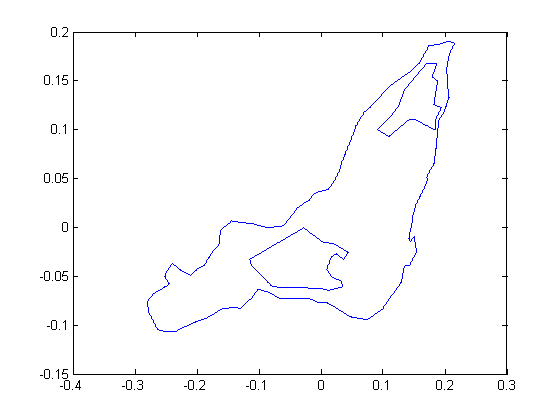
\includegraphics[width=3.5in]{figs/mtl_geometry.png}

P. E. Trudeau airport and the rail yards,  and the oil refineries
and water treatment plant are removed.

\end{frame}

%  ---------------------------------------------------------------------

%  ---------------------------------------------------------------------
%  ---------------------------------------------------------------------

\section{Some notation: Two partial differentiation operators}

\begin{frame}

\bi
  \item Function $u$ is the solution of a \emph{partial differential equation}.
  \item That is, it is defined in terms of an equation relating derivatives
  with respect $x$, $y$ and $t$.
  \item These equations can be expressed quite simply in terms of two types of
  partial derivatives.
\ei

\end{frame}

%  ---------------------------------------------------------------------

\begin{frame}

We need the ``grad'' operator $\nabla$, which stands for the
operation of calculating the gradient.  That is,
\[
  \nabla = \left[
  \begin{array}{c}
  \frac{\partial}{\partial x}  \\ \\
  \frac{\partial}{\partial y}
  \end{array}
  \right]
\]
so that
\[
  \nabla u = \left[
  \begin{array}{c}
  \frac{\partial u}{\partial x} \nonumber \\ \\
  \frac{\partial u}{\partial y}
  \end{array}
  \right].
\]

The ``Laplacian'' operator $\triangle$ can be expressed as $\nabla
\cdot \nabla$ and also as $\nabla^2$:
\[
  \triangle u = \nabla^2 u = \frac{\partial^2 u}{\partial x^2}  +
  \frac{\partial^2 u}{\partial y^2}
\]

\end{frame}

%  ---------------------------------------------------------------------

%  ---------------------------------------------------------------------
%  ---------------------------------------------------------------------

\section{The equations solved by Matlab's pde toolbox}

\begin{frame}

The core task of the PDE toolbox is to solve equations of the
form:

\begin{eqnarray}
  -\nabla \cdot (\Cbold \nabla u) + a u & = & f
  \nonumber \\
  d \frac{du}{dt} -\nabla \cdot (\Cbold \nabla u) + a u & = & f
  \nonumber \\
  d \frac{du^2}{d^2t} -\nabla \cdot (\Cbold \nabla u) + a u & = & f
  \nonumber \\
\end{eqnarray}

Scalars $a, f$, and $d$; and 2 by 2 matrix $\Cbold$ can be either
constants or functions of $t, x,$ and $y$.

\end{frame}

%  ---------------------------------------------------------------------

\begin{frame}

\frametitle{Interpreting the equations: time dependency}

\bi
  \item You can separate the time-dependent behavior from the
  spatially-dependent behavior.
  \item The first equation, called ``elliptic'', has no
  time-dependency.
  \item The second equation, called ``parabolic'', has first-order
  time-dependency, and therefore shows either linear or exponential
  decay or growth with respect to time.
  \item The second equation, called ``hyperbolic'', has second-order
  time-dependency, and therefore shows sinusoidal oscillation
  with respect to time.
  \item Each of the equations is \emph{forced} by exogenous input
  represented by function $f$.
\ei

\end{frame}

%  ---------------------------------------------------------------------

\begin{frame}


\frametitle{The second-order spatial dependency}

\bi
  \item These equations all involve second derivative or curvature
  variation over space.
  \item If $\Cbold$ is constant, the curvature does not vary, and
  the spatial variation is \emph{isotropic}.
  \item If $\Cbold$ is a function, then curvature varies from
  location to location, and possibly over time as well, and is
  \emph{anisotropic}.
\ei

\end{frame}

%  ---------------------------------------------------------------------

\begin{frame}


\frametitle{The interaction between temporal and spatial variation}

\bi
  \item You can think of these equations as ordinary differential
  equations in time $t$ forced by spatial curvature.
  \item Let's look at the parabolic equation with constant
  curvature coefficient $c$ and $f = 0$, taking spatial curvature over to the
  forcing side:
  \[
    d \frac{du}{dt} = -au
        + c \nabla \cdot \nabla u = -au + c \triangle u
  \]
  \item  The local rate of change in $u$ over $t$ is
  proportional to the curvature.
\ei

\end{frame}

%  ---------------------------------------------------------------------

\begin{frame}


  \[
    d \frac{du}{dt} = =au +
        c \nabla \cdot \nabla u = -au + c \triangle u
  \]

\bi
  \item  If curvature is sharply negative at a location,
  such as at a peak, $u$ will decay at that location.
  \item  Where the curvature is sharply positive, in
  a valley or a well, $u$ will increase over time.
  \item  This happens when something \emph{diffuses}, so
  that high concentrations at a point diffuse outwards, and
  local low concentrations are increased by inward diffusion.
  \item This equation is called the \emph{heat} or \emph{diffusion}
  equation.
\ei

\end{frame}

%  ---------------------------------------------------------------------

\begin{frame}


\frametitle{Income in the Island of Montreal}

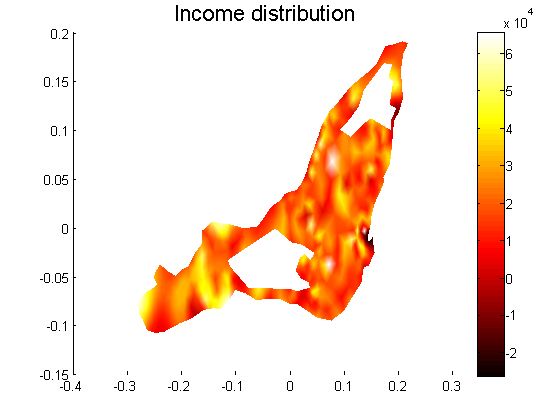
\includegraphics[width=3.5in]{figs/mtlwealth.png}

\end{frame}

%  ---------------------------------------------------------------------

\begin{frame}


\frametitle{A socialist scenario}

\bi
  \item Quebec separates from Canada, and an aggressively leftist
  government takes over the legislature.
  \item Premier Fid\`ele Castreau and his finance minister,
  Jacques L\'eton bring in measures to help the rich share their
  income with the poor, which they enthusiastically agree to.
  \item What will happen?
\ei

\end{frame}

%  ---------------------------------------------------------------------

\begin{frame}


\frametitle{Elliptic or steady-state equations and hyperbolic or wave equations}

\bi
  \item If we replace $du/dt$ in the heat equation by 0, we
  get the final steady-state that a diffusion process
  tends to.
  \item On the other hand, if we replace $du/dt$ by $d^2u/dt^2$
  we get the basic linear or exponential decay replaced by
  oscillation, and this is the \emph{wave} equation.
  \item In either case, the long-term behavior of $u$
  depends on what is happening at the boundaries.
  \item Let's look at boundary behavior next.
\ei

\end{frame}

%  ---------------------------------------------------------------------

%  ---------------------------------------------------------------------
%  ---------------------------------------------------------------------

\section{Boundary behavior}

\begin{frame}

\frametitle{Fixed boundary behavior}

\bi
  \item Here are two scenarios.
  \item Rich people tend to live near the water on the Island of
  Montreal.
  \item Perhaps these people will insist that their income be left
  fixed.  Leave it to the people who live in the interior to
  diffuse their income around.
  \item Fixing the boundaries is called a \emph{Dirichlet} boundary
  condition.
  \[
    hu = r \ \ \mbox{on} \ \ \partial \Omega
  \]
  where $h$ and $r$ can be constants or functions.
\ei

\end{frame}

%  ---------------------------------------------------------------------

\begin{frame}


\frametitle{Fixed flow across the boundary}

\bi
  \item On the other hand, perhaps the government will put a wall
  around the island, so that money can neither enter nor leave.
  The diffusion across the boundary will be zero.
  \item This is called a \emph{Neumann} boundary condition.
  \[
    \nbold \cdot(\Cbold \nabla u) + q u = g
     \ \ \mbox{on} \ \ \partial \Omega
  \]
  where $\nbold$ is the normal vector on the boundary,
  and $g$ is the flow rate across the boundary.
  \item Mixtures of these conditions are also possible.
\ei

\end{frame}

%  ---------------------------------------------------------------------

%  ---------------------------------------------------------------------
%  ---------------------------------------------------------------------

\section{Income diffusion with zero boundary flow}

\begin{frame}

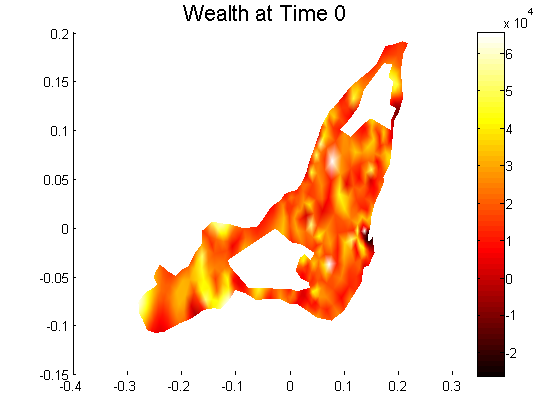
\includegraphics[width=3.5in]{figs/mtl_0.png}

Hampstead has six times the income of Snowdon.

\end{frame}

%  ---------------------------------------------------------------------

\begin{frame}

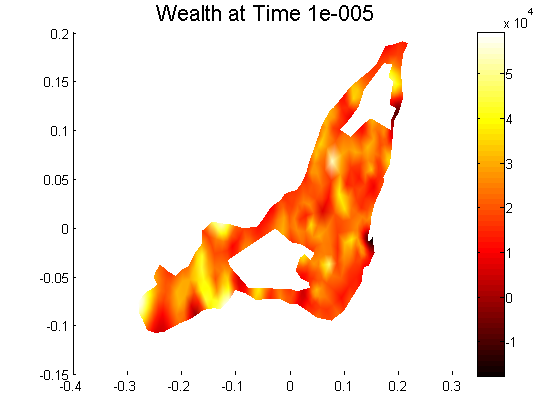
\includegraphics[width=3.5in]{figs/mtl_1e-5.png}

Things are improving; Hampstead has only four times the income of
its neighbors.

\end{frame}

%  ---------------------------------------------------------------------

\begin{frame}


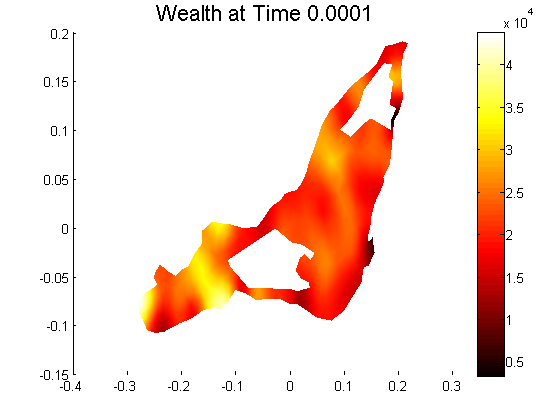
\includegraphics[width=3.5in]{figs/mtl_1e-4.png}

Near-justice on the mountain, but Beaconsfield has three times the
income of Lachine.

\end{frame}

%  ---------------------------------------------------------------------

\begin{frame}


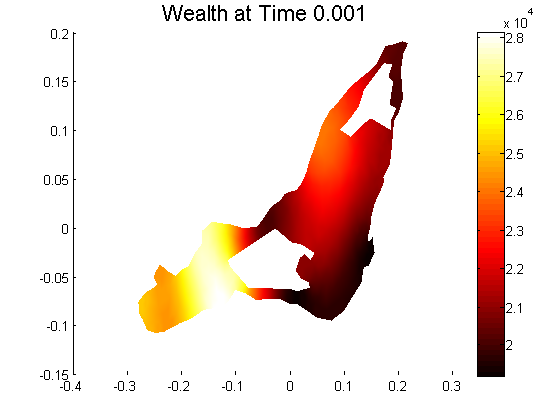
\includegraphics[width=3.5in]{figs/mtl_1e-3.png}

Income variation is now much smaller, but income is still piling
up behind the airport and rail yards.

\end{frame}

%  ---------------------------------------------------------------------

\begin{frame}

\frametitle{Spatial smoothing with the heat equation}

\bi
  \item The parabolic equation combined with the Neumann boundary
  condition gives a recipe for spatial smoothing.
  \item Time $t$ plays the role of the smoothing parameter
  $\lambda$ in smoothing with a roughness penalty.
  \item $\triangle u$ plays the role of the roughness penalty.
  It corresponds to penalty $\int [Dx(t)]^2 \, dt$.  You can
  go from one to the other by integrating by parts.
  \item The final steady state is a constant, and hence
  this closely resembles kernel smoothing as well.
  \item But the Neumann boundary condition plays a key role:
  it prevents stuff crossing the boundaries.  In this case,
  income cannot cross the airport to get to the other side.
  Kernel and roughness penalty methods cannot achieve this.
\ei

\end{frame}

%  ---------------------------------------------------------------------

%  ---------------------------------------------------------------------
%  ---------------------------------------------------------------------

\section{How does PDE toolbox work?}

\begin{frame}

\frametitle{Specifying boundaries}

\bi
  \item Boundaries are specified by line and arc segments.
  \item Boundary information is often available in
  geographical information system (GIS) databases.  I got these
  boundaries from the Geography library.
  \item Boundary conditions can be specified separately for each
  boundary segment.
\ei

\end{frame}

%  ---------------------------------------------------------------------

\begin{frame}

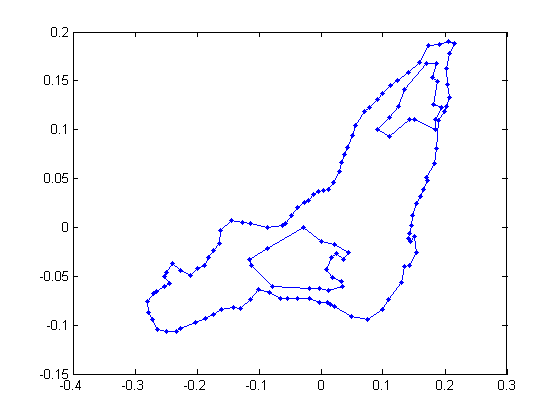
\includegraphics[width=3.5in]{figs/mtlboundary.png}

The outside boundary has 1110 linear segments.

\end{frame}

%  ---------------------------------------------------------------------

\begin{frame}


\frametitle{The interior triangular mesh}

\bi
  \item The interior is divided into triangles.
  \item The sizes of the triangles are adjusted so
  as to have smaller triangles where things are changing
  quickly or are spatially complex.
  \item About 90\% of the computational cleverness in the toolbox
  is associated with getting a good mesh.
\ei

\end{frame}

%  ---------------------------------------------------------------------

\begin{frame}


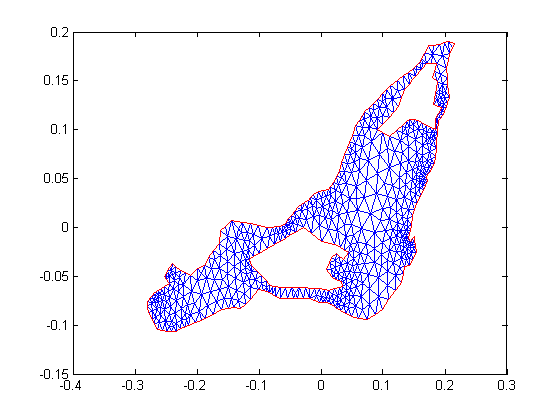
\includegraphics[width=3.5in]{figs/mtl_mesh.png}

There are 1063 triangles covering the area to be smoothed. They
meet at 664 vertices and are defined by 267 edges.

\end{frame}

%  ---------------------------------------------------------------------

\begin{frame}

\frametitle{Census tracts in the Island of Montreal}

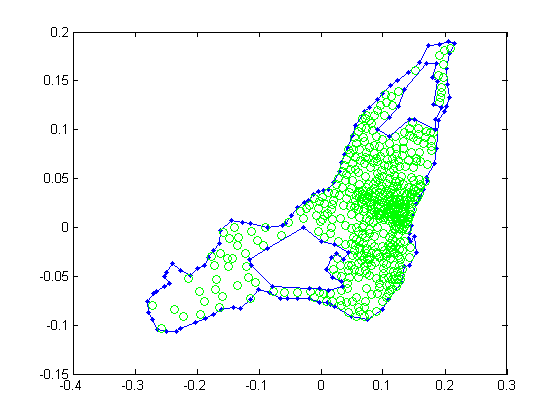
\includegraphics[width=3.5in]{figs/mtlcensus.png}

There were 493 census tracts on the Island.

\end{frame}

%  ---------------------------------------------------------------------

\begin{frame}


\frametitle{Interpolating the information on to the triangular mesh}

\bi
  \item The irregularly spaced census income values are
  interpolated to a rectangular grid.
  \item Each triangle vertex is assigned the income value of
  the rectangle containing the vertex.
  \item This becomes the state of the system at time $t = 0.$
\ei

\end{frame}

%  ---------------------------------------------------------------------

\begin{frame}


\frametitle{Finite element basis functions}

\bi
  \item A piece-wise linear basis function is associated
  with each vertex.
  \item Each interior basis function is nonzero over an irregular
  hexagon composed of the six triangles that meet at that
  vertex.  Exterior basis functions will have fewer triangular
  components.
  \item The basis function is linear everywhere, zero on its
  exterior boundary, and has value 1 at its central vertex.  It looks
  like a tent.
  \item The coefficient multiplying each basis function is
  simply the value of the data at the central vertex.
\ei

\end{frame}

%  ---------------------------------------------------------------------

%  ---------------------------------------------------------------------
%  ---------------------------------------------------------------------

\section{Solving the equation}

\begin{frame}

\bi
  \item The differential equation is converted to an
  equivalent integral equation, and
  \item this equation is in turn
  equivalent to a linear equation in the coefficients.
  \item The linear system is usually huge, but most
  of the elements of the coefficient matrix are zero.
  Typically only 5\% or so are not.  The system is
  solved using sparse matrix computation methods.
\ei

\end{frame}

%  ---------------------------------------------------------------------

%  ---------------------------------------------------------------------
%  ---------------------------------------------------------------------

\section{How do I get into all this?}

\begin{frame}

\bi
  \item Begin by using the graphical interface for the PDE
  toolbox.
  \item To activate it, type \texttt{pdetool} into the Matlab
  command window.
  \item Work through some of the examples in the manual that comes
  with the tool box
\ei

\end{frame}

\end{document}
